\documentclass[12pt]{report}
\usepackage[utf8]{inputenc}
\usepackage[T2A]{fontenc}
\usepackage[russian]{babel}

\usepackage{amsmath,amsfonts,amssymb,amsthm,mathtools}
\DeclarePairedDelimiter\abs{\lvert}{\rvert}

\usepackage{pgfplots}
\usepackage{filecontents}
\usepackage{indentfirst}
\usepackage{eucal}
\usepackage{enumitem}
% Для \abs{}
\usepackage{commath}
\usepackage{float}
\frenchspacing

% Для нормальных переносов
\sloppy

\usetikzlibrary{datavisualization}
\usetikzlibrary{datavisualization.formats.functions}

\usepackage[left=2cm,right=2cm, top=2cm,bottom=2cm,bindingoffset=0cm]{geometry}
% Для измененных титулов глав:
\usepackage{titlesec, blindtext, color} % подключаем нужные пакеты
\definecolor{gray75}{gray}{0.75} % определяем цвет
\newcommand{\hsp}{\hspace{20pt}} % длина линии в 20pt
% titleformat определяет стиль
\titleformat{\chapter}[hang]{\Huge\bfseries}{\thechapter\hsp\textcolor{gray75}{|}\hsp}{0pt}{\Huge\bfseries}

% plot
\usepackage{xcolor}
\usepackage{stmaryrd}
\usepackage{wasysym}
\usetikzlibrary{datavisualization}
\usetikzlibrary{datavisualization.formats.functions}

% листинги
\usepackage{listings}
\usepackage{graphicx}
\usepackage{caption}
\usepackage{textcomp}
\lstset{
    language = Python,
    basicstyle=\small\sffamily,
    numbers=left,
    numberstyle=\tiny,
    stepnumber=1,
    numbersep=5pt,
    showspaces=false,
    showstringspaces=false,
    showtabs=false,
    frame=single,
    tabsize=2,
    captionpos=t,
    breaklines=true,
    breakatwhitespace=false,
    escapeinside={\#*}{*)},
    literate=	{а}{{\selectfont\char224}}1
			    {б}{{\selectfont\char225}}1
			    {в}{{\selectfont\char226}}1
			    {г}{{\selectfont\char227}}1
			    {д}{{\selectfont\char228}}1
			    {е}{{\selectfont\char229}}1
			    {ё}{{\"e}}1
			    {ж}{{\selectfont\char230}}1
			    {з}{{\selectfont\char231}}1
			    {и}{{\selectfont\char232}}1
			    {й}{{\selectfont\char233}}1
			    {к}{{\selectfont\char234}}1
			    {л}{{\selectfont\char235}}1
			    {м}{{\selectfont\char236}}1
			    {н}{{\selectfont\char237}}1
			    {о}{{\selectfont\char238}}1
			    {п}{{\selectfont\char239}}1
			    {р}{{\selectfont\char240}}1
			    {с}{{\selectfont\char241}}1
			    {т}{{\selectfont\char242}}1
			    {у}{{\selectfont\char243}}1
			    {ф}{{\selectfont\char244}}1
			    {х}{{\selectfont\char245}}1
			    {ц}{{\selectfont\char246}}1
			    {ч}{{\selectfont\char247}}1
			    {ш}{{\selectfont\char248}}1
			    {щ}{{\selectfont\char249}}1
			    {ъ}{{\selectfont\char250}}1
			    {ы}{{\selectfont\char251}}1
			    {ь}{{\selectfont\char252}}1
			    {э}{{\selectfont\char253}}1
			    {ю}{{\selectfont\char254}}1
			    {я}{{\selectfont\char255}}1
			    {А}{{\selectfont\char192}}1
			    {Б}{{\selectfont\char193}}1
			    {В}{{\selectfont\char194}}1
			    {Г}{{\selectfont\char195}}1
			    {Д}{{\selectfont\char196}}1
			    {Е}{{\selectfont\char197}}1
			    {Ё}{{\"E}}1
			    {Ж}{{\selectfont\char198}}1
			    {З}{{\selectfont\char199}}1
			    {И}{{\selectfont\char200}}1
			    {Й}{{\selectfont\char201}}1
			    {К}{{\selectfont\char202}}1
			    {Л}{{\selectfont\char203}}1
			    {М}{{\selectfont\char204}}1
			    {Н}{{\selectfont\char205}}1
			    {О}{{\selectfont\char206}}1
			    {П}{{\selectfont\char207}}1
			    {Р}{{\selectfont\char208}}1
			    {С}{{\selectfont\char209}}1
			    {Т}{{\selectfont\char210}}1
			    {У}{{\selectfont\char211}}1
			    {Ф}{{\selectfont\char212}}1
			    {Х}{{\selectfont\char213}}1
			    {Ц}{{\selectfont\char214}}1
			    {Ч}{{\selectfont\char215}}1
			    {Ш}{{\selectfont\char216}}1
			    {Щ}{{\selectfont\char217}}1
			    {Ъ}{{\selectfont\char218}}1
			    {Ы}{{\selectfont\char219}}1
			    {Ь}{{\selectfont\char220}}1
			    {Э}{{\selectfont\char221}}1
			    {Ю}{{\selectfont\char222}}1
			    {Я}{{\selectfont\char223}}1
			    {№}{{\selectfont N}}1
}
\captionsetup[lstlisting]{justification=raggedright, singlelinecheck=off}

\addto\captionsrussian{% Replace "english" with the language you use
	\renewcommand{\contentsname}%
	{Содержание	}%
}

\begin{document}
	% Титульник
\thispagestyle{empty}
\begin{titlepage}
	\noindent \begin{minipage}{0.15\textwidth}
		
\includegraphics[width=\linewidth]{img/b-logo}
	\end{minipage}
	\noindent\begin{minipage}{0.9\textwidth}
		\centering
		\textbf{Министерство науки и высшего образования Российской Федерации}\\
		\textbf{Федеральное государственное бюджетное образовательное учреждение высшего образования}\\
		\textbf{~~~«Московский государственный технический университет имени Н.Э.~Баумана}\\
		\textbf{(национальный исследовательский университет)»}\\
		\textbf{(МГТУ им. Н.Э.~Баумана)}
	\end{minipage}
	
	\noindent\rule{18cm}{3pt}
	\newline\newline
	\noindent ФАКУЛЬТЕТ $\underline{\text{«Информатика и системы управления»}}$ \newline\newline
	\noindent КАФЕДРА $\underline{\text{«Программное обеспечение ЭВМ и информационные технологии»}}$\newline\newline\newline\newline\newline
	
	
	\begin{center}
		\noindent\begin{minipage}{1.3\textwidth}
			\centering
			\Large\textbf{  Отчет по лабораторной работе №3}\newline
			\textbf{по дисциплине "Анализ алгоритмов"}\newline\newline
		\end{minipage}
	\end{center}
	
	\noindent\textbf{Тема} $\underline{\text{Сравнительный анализ алгоритмов сортировки}}$\newline\newline
	\noindent\textbf{Студент} $\underline{\text{Шацкий Р.Е.}}$\newline\newline
	\noindent\textbf{Группа} $\underline{\text{ИУ7-55Б}}$\newline\newline
	\noindent\textbf{Оценка (баллы)} $\underline{\text{~~~~~~~~~~~~~~~~~~~~~~~~~~~}}$\newline\newline
	\noindent\textbf{Преподаватели} $\underline{\text{Волкова Л.Л., Строганов Ю.В.}}$\newline\newline\newline
	
	\begin{center}
		\vfill
		Москва~---~\the\year
		~г.
	\end{center}
\end{titlepage}
	\pagenumbering{arabic}
	\newpage
	\tableofcontents
%\def\chaptername{} % убирает "Глава"
	\addcontentsline{toc}{chapter}{Введение}
    \chapter*{Введение}
    Конвейер\cite{conveyor} — способ организации вычислений, используемый в современных процессорах и контроллерах с целью повышения их производительности (увеличения числа инструкций, выполняемых в единицу времени — эксплуатация параллелизма на уровне инструкций), технология, используемая при разработке компьютеров и других цифровых электронных устройств.
    
    Сам термин <<конвейер>> пришёл из промышленности, где используется подобный принцип работы — материал автоматически подтягивается по ленте конвейера к рабочему, который осуществляет с ним необходимые действия, следующий за ним рабочий выполняет свои функции над получившейся заготовкой, следующий делает ещё что-то. Таким образом, к концу конвейера цепочка рабочих полностью выполняет все поставленные задачи, сохраняя высокий темп производства. Например, если на самую медленную операцию затрачивается одна минута, то каждая деталь будет сходить с конвейера через одну минуту. В процессорах роль рабочих исполняют функциональные модули, входящие в состав процессора.
    
    
    \textbf{Целью данной работы} является реализация асинхронного взаимодействия потоков на примере конвейерной обработки данных.
    
    Для достижения поставленной цели необходимо выполнить следующие \textbf{задачи:}
    \begin{enumerate}
    	\item Изучить асинхронное взаимодействие на примере конвейерной обработки данных.
    	\item Привести схему конвейерных вычислений.
    	\item Описать используемые структуры данных.
    	\item Определить средства программной реализации.
    	\item Реализовать и протестировать ПО.
    	\item Провести сравнительный последовательной и конвейерной реализации по затрачиваемым ресурсам (времени работы).
    	\item Изучить время, затрачиваемое на нахождение заявки в очереди к каждому этапу конвейера.
    \end{enumerate}
    \newpage
    
    \chapter{Аналитическая часть}	
    В данном разделе рассматриваются принципы и идея конвейерной обработки данных, а также приводится описание решаемой задачи и выделенных стадий конвейерной обработки.
    
    \section{Описание конвейерной обработки данных}
    Конвейер\cite{conveyor} — способ организации вычислений, используемый в современных процессорах и контроллерах с целью повышения их производительности (увеличения числа инструкций, выполняемых в единицу времени — эксплуатация параллелизма на уровне инструкций), технология, используемая при разработке компьютеров и других цифровых электронных устройств.
    
    Идея заключается в параллельном выполнении нескольких инструкций процессора. Сложные инструкции процессора представляются в виде последовательности более простых стадий. Вместо выполнения инструкций последовательно (ожидания завершения конца одной инструкции и перехода к следующей), следующая инструкция может выполняться через несколько стадий выполнения первой инструкции. Это позволяет управляющим цепям процессора получать инструкции со скоростью самой медленной стадии обработки, однако при этом намного быстрее, чем при выполнении эксклюзивной полной обработки каждой инструкции от начала до конца.
    
    Многие современные процессоры управляются тактовым генератором. Процессор внутри состоит из логических элементов и ячеек памяти — триггеров. Когда приходит сигнал от тактового генератора, триггеры приобретают своё новое значение, и «логике» требуется некоторое время для декодирования новых значений. Затем приходит следующий сигнал от тактового генератора, триггеры принимают новые значения, и так далее. Разбивая последовательности логических элементов на более короткие и помещая триггеры между этими короткими последовательностями, уменьшают время, необходимое логике для обработки сигналов. В этом случае длительность одного такта процессора может быть соответственно уменьшена.
    
    \section{Выделенные стадии конвейерной обработки}
    В данной работе в качестве алгоритма, реализованного для конвейеризации, используется шифрование паролей с сохранением в базу данных. Таким образом, было выделено три ленты конвейера:
    \begin{enumerate}
    	\item Загрузка логинов и паролей из базы данных.
    	\item Многократное последовательное хеширование полученной строки для большей безопасности.
    	\item Загрузка полученного значения в базу данных.
    \end{enumerate}
    \subsection{Загрузка логинов и паролей из базы данных}
    Изначальные логины пользователей и пароли для хеширования загружаются из базы данных.
    
    \subsection{Многократное последовательное хеширование}
    Существует много алгоритмов хеш-шифрования данных, наиболее распространенные из них приведены ниже \cite{hashes}.
    \begin{enumerate}
    	\item MD5 - алгоритм дайджеста сообщений (Message-Digest algorithm), генерирует 128-битное хэш-значение; не может предотвратить коллизии и, следовательно, может быть взломан.
    	\item SHA-1 - Secure Hash Algorithm 1, может генерировать дайджест сообщения - 160-битное хеш-значение, обычная форма - 40 шестнадцатеричных чисел; не является достаточно безопасным, был обнаружен эффективного метод атаки.
    	\item SHA-2/SHA-256 - Secure Hash Algorithm 2, генерирует 256-битное хеш-значение; существуют алгоритмы SHA-224, SHA-384, SHA-512, названия которых содержат двоичную длину SHA-2.
    	\item HMAC - Hash-based Message Authentication Code, использует алгоритм хеширования, принимает сообщение M и ключ K в качестве входных данных и генерирует дайджест сообщения фиксированной длины в качестве выходных данных.
    \end{enumerate}
    
    Использование однократного хеширования потенциально небезопасно по нескольким причинам \cite{security}:
    \begin{itemize}
    	\item существование коллизий - при одинаковых паролях хеш-значения будут совпадать;
    	\item существование таблиц хэшей для различных функций.
    \end{itemize}
    
    Существует несколько способов увеличения надежности хеш-функций \cite{security}:
    \begin{enumerate}
    	\item использование "соли" - добавление символьной последовательности в конец строки;
    	\item использование нескольких этапов хеширования, использующих разные хеш-функции;
    	\item растяжение пароля - итеративный, или рекурсивный, алгоритм, который вычисляет хэш самого себя большое количество раз (на каждом этапе к значению добавляется новая "соль").
    \end{enumerate}
    
    В данной работе для обеспечения безопасности хранения данных используется хеш-функция SHA-512 и способ растяжения паролей.
    
    \subsection{Загрузка в базу данных}
    По завершении всех предыдущих этапов обработанные пароли пользователей заносятся в локальную реляционную базу данных.
    
    \section{Требования к программному обеспечению}
    На основе приведенного алгоритма можно выдвинуть требования к разрабатываемому ПО:
    \begin{itemize}
    	%	\item входные данные - размер матрицы (целое число), её элементы (вещественные числа, по желанию пользователя, в противном случае - генерация произвольной матрицы заданного размера);
    	\item выходные данные - время работы последовательного выполнения действий (вещественное число);
    	\item время работы конвейера (вещественное число);
    	\item минимальное, среднее, максимальное времена ожидания заявки в очереди каждой из конвейерных лент (вещественные числа);
    	\item наличие обработки некорректного ввода.
    \end{itemize}
    
    \section{Вывод}
    Был рассмотрен алгоритм шифрования пароля пользователя и его сохранение в базу данных.
    Были рассмотрены шаги алгоритма шифрования, выполняемые каждой лентой конвейера для оптимизации работы алгоритма.
    Выдвинуты требования к разрабатываемому ПО: выходные данные (включающие в себя время работы конвейера, минимальное, среднее, а также максимальное время ожидания заявки в очереди) и наличие обработки некорректного ввода.
    
    \newpage
    
    \chapter{Конструкторская часть}
    Данный раздел содержит схемы конвейерной обработки данных, последовательного и конвейерного алгоритма.
    
    \section{Схемы алгоритмов}
    В данном пункте раздела представлены схемы реализуемых в работе алгоритмов.
    
    На рисунке~\ref{img:conveer} представлена схема организации конвейерных вычислений на примере конвейера с тремя лентами.
    \begin{figure}[H]
    	\centering
    	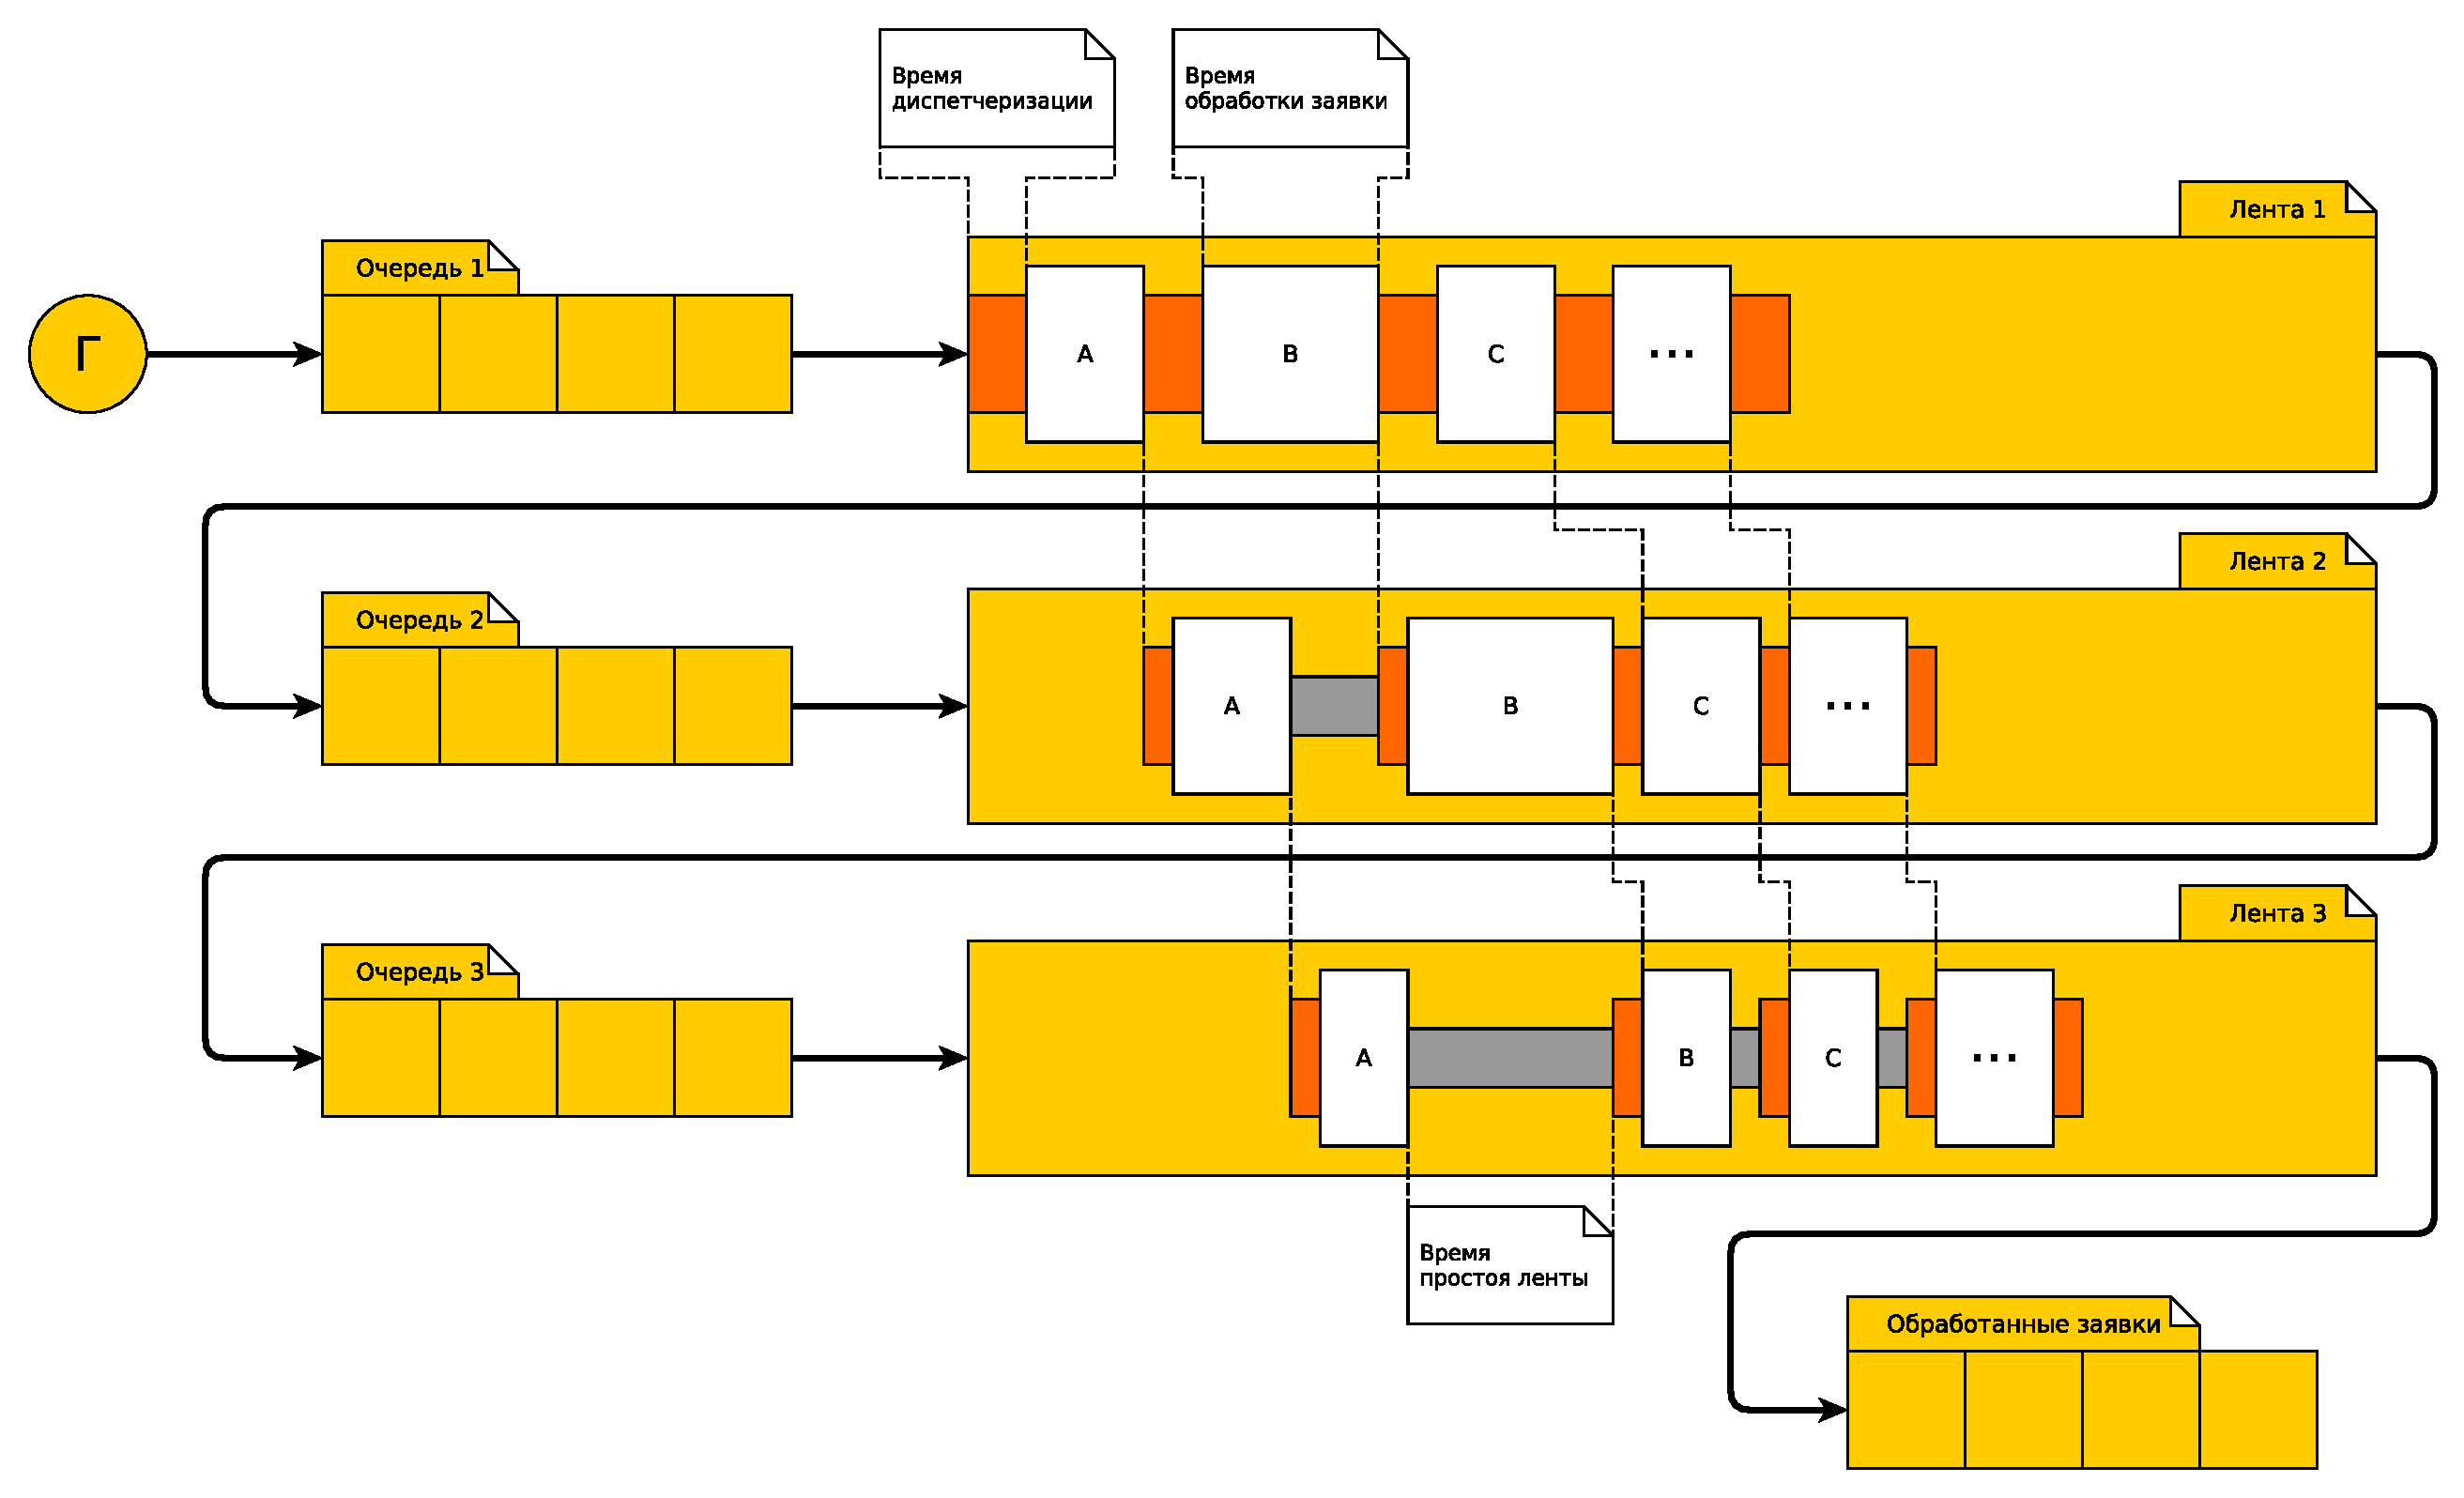
\includegraphics[width=1.00\linewidth]{img/conveer}
    	\caption{Схема организации конвейера с тремя лентами}
    	\label{img:conveer}
    \end{figure}
    %
    %На рисунке~\ref{img:thread_schema} представлена схема последовательного алгоритма шифрования и сохранения паролей.
    %
    %\begin{figure}[H]
    %	\centering
    %	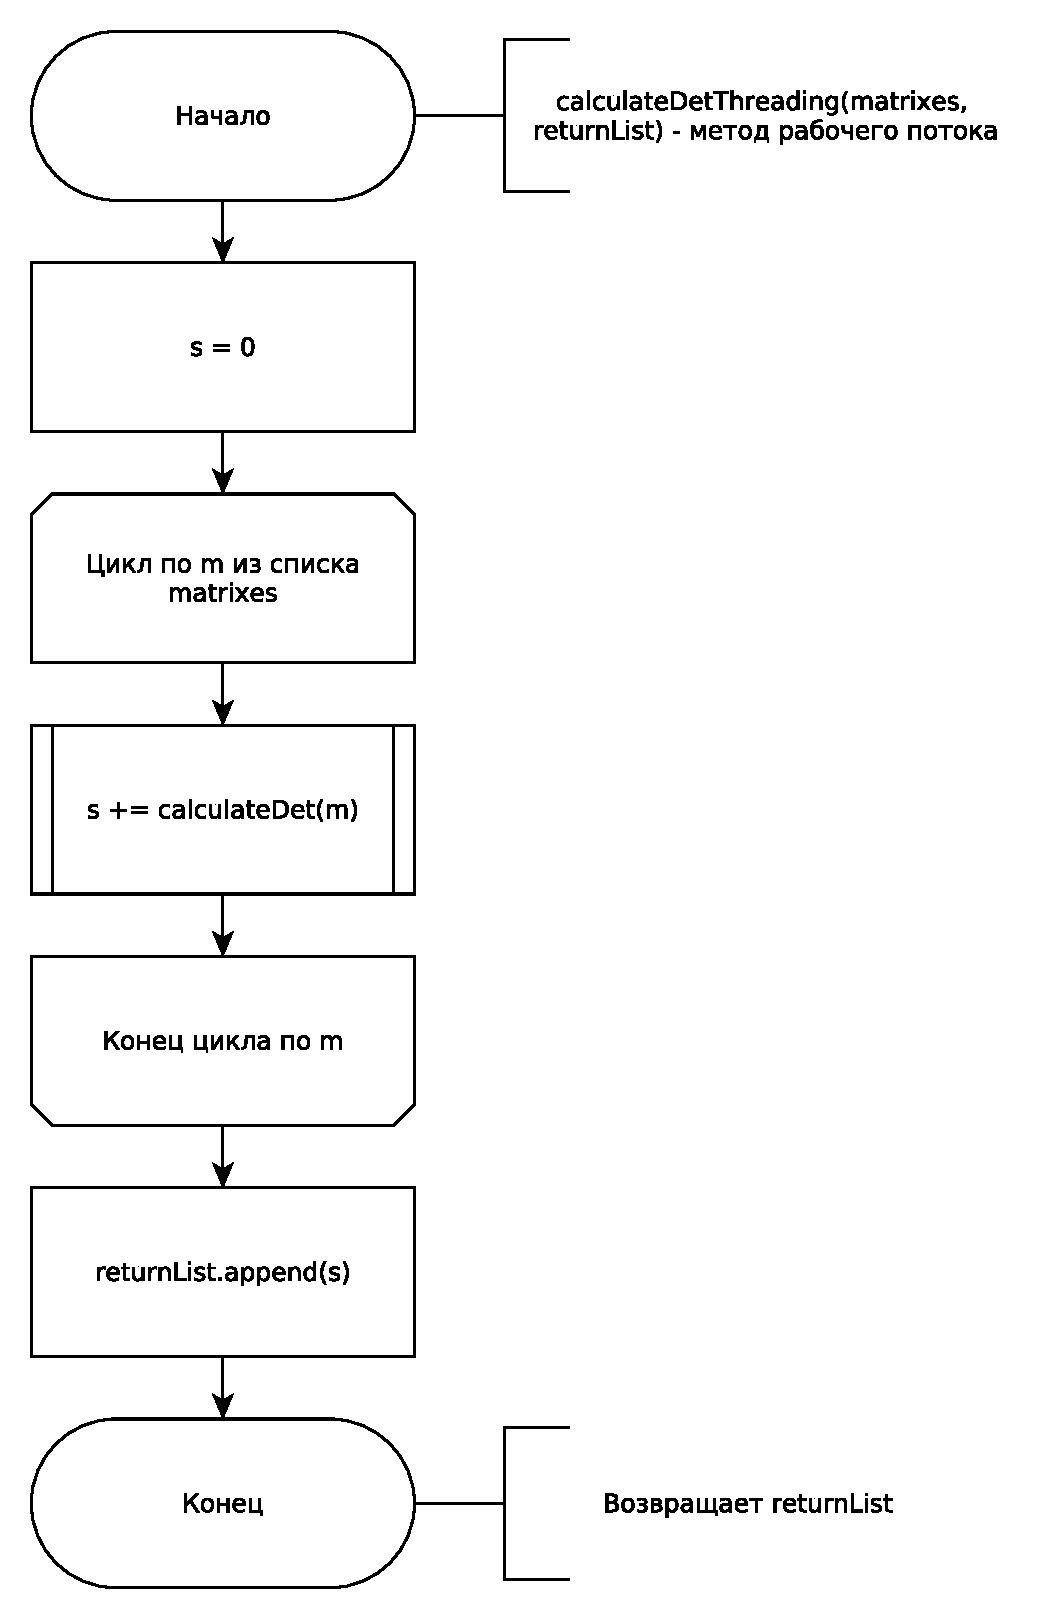
\includegraphics[width=0.85\linewidth]{img/thread_schema}
    %	\caption{Схема последовательного алгоритма}
    %	\label{img:thread_schema}
    %\end{figure}
    %
    %На рисунках~\ref{img:solver_1} -~\ref{img:solver_2} представлена схема реализация алгоритма шифрования на конвейере с тремя лентами.
    %
    %\begin{figure}[H]
    %	\centering
    %	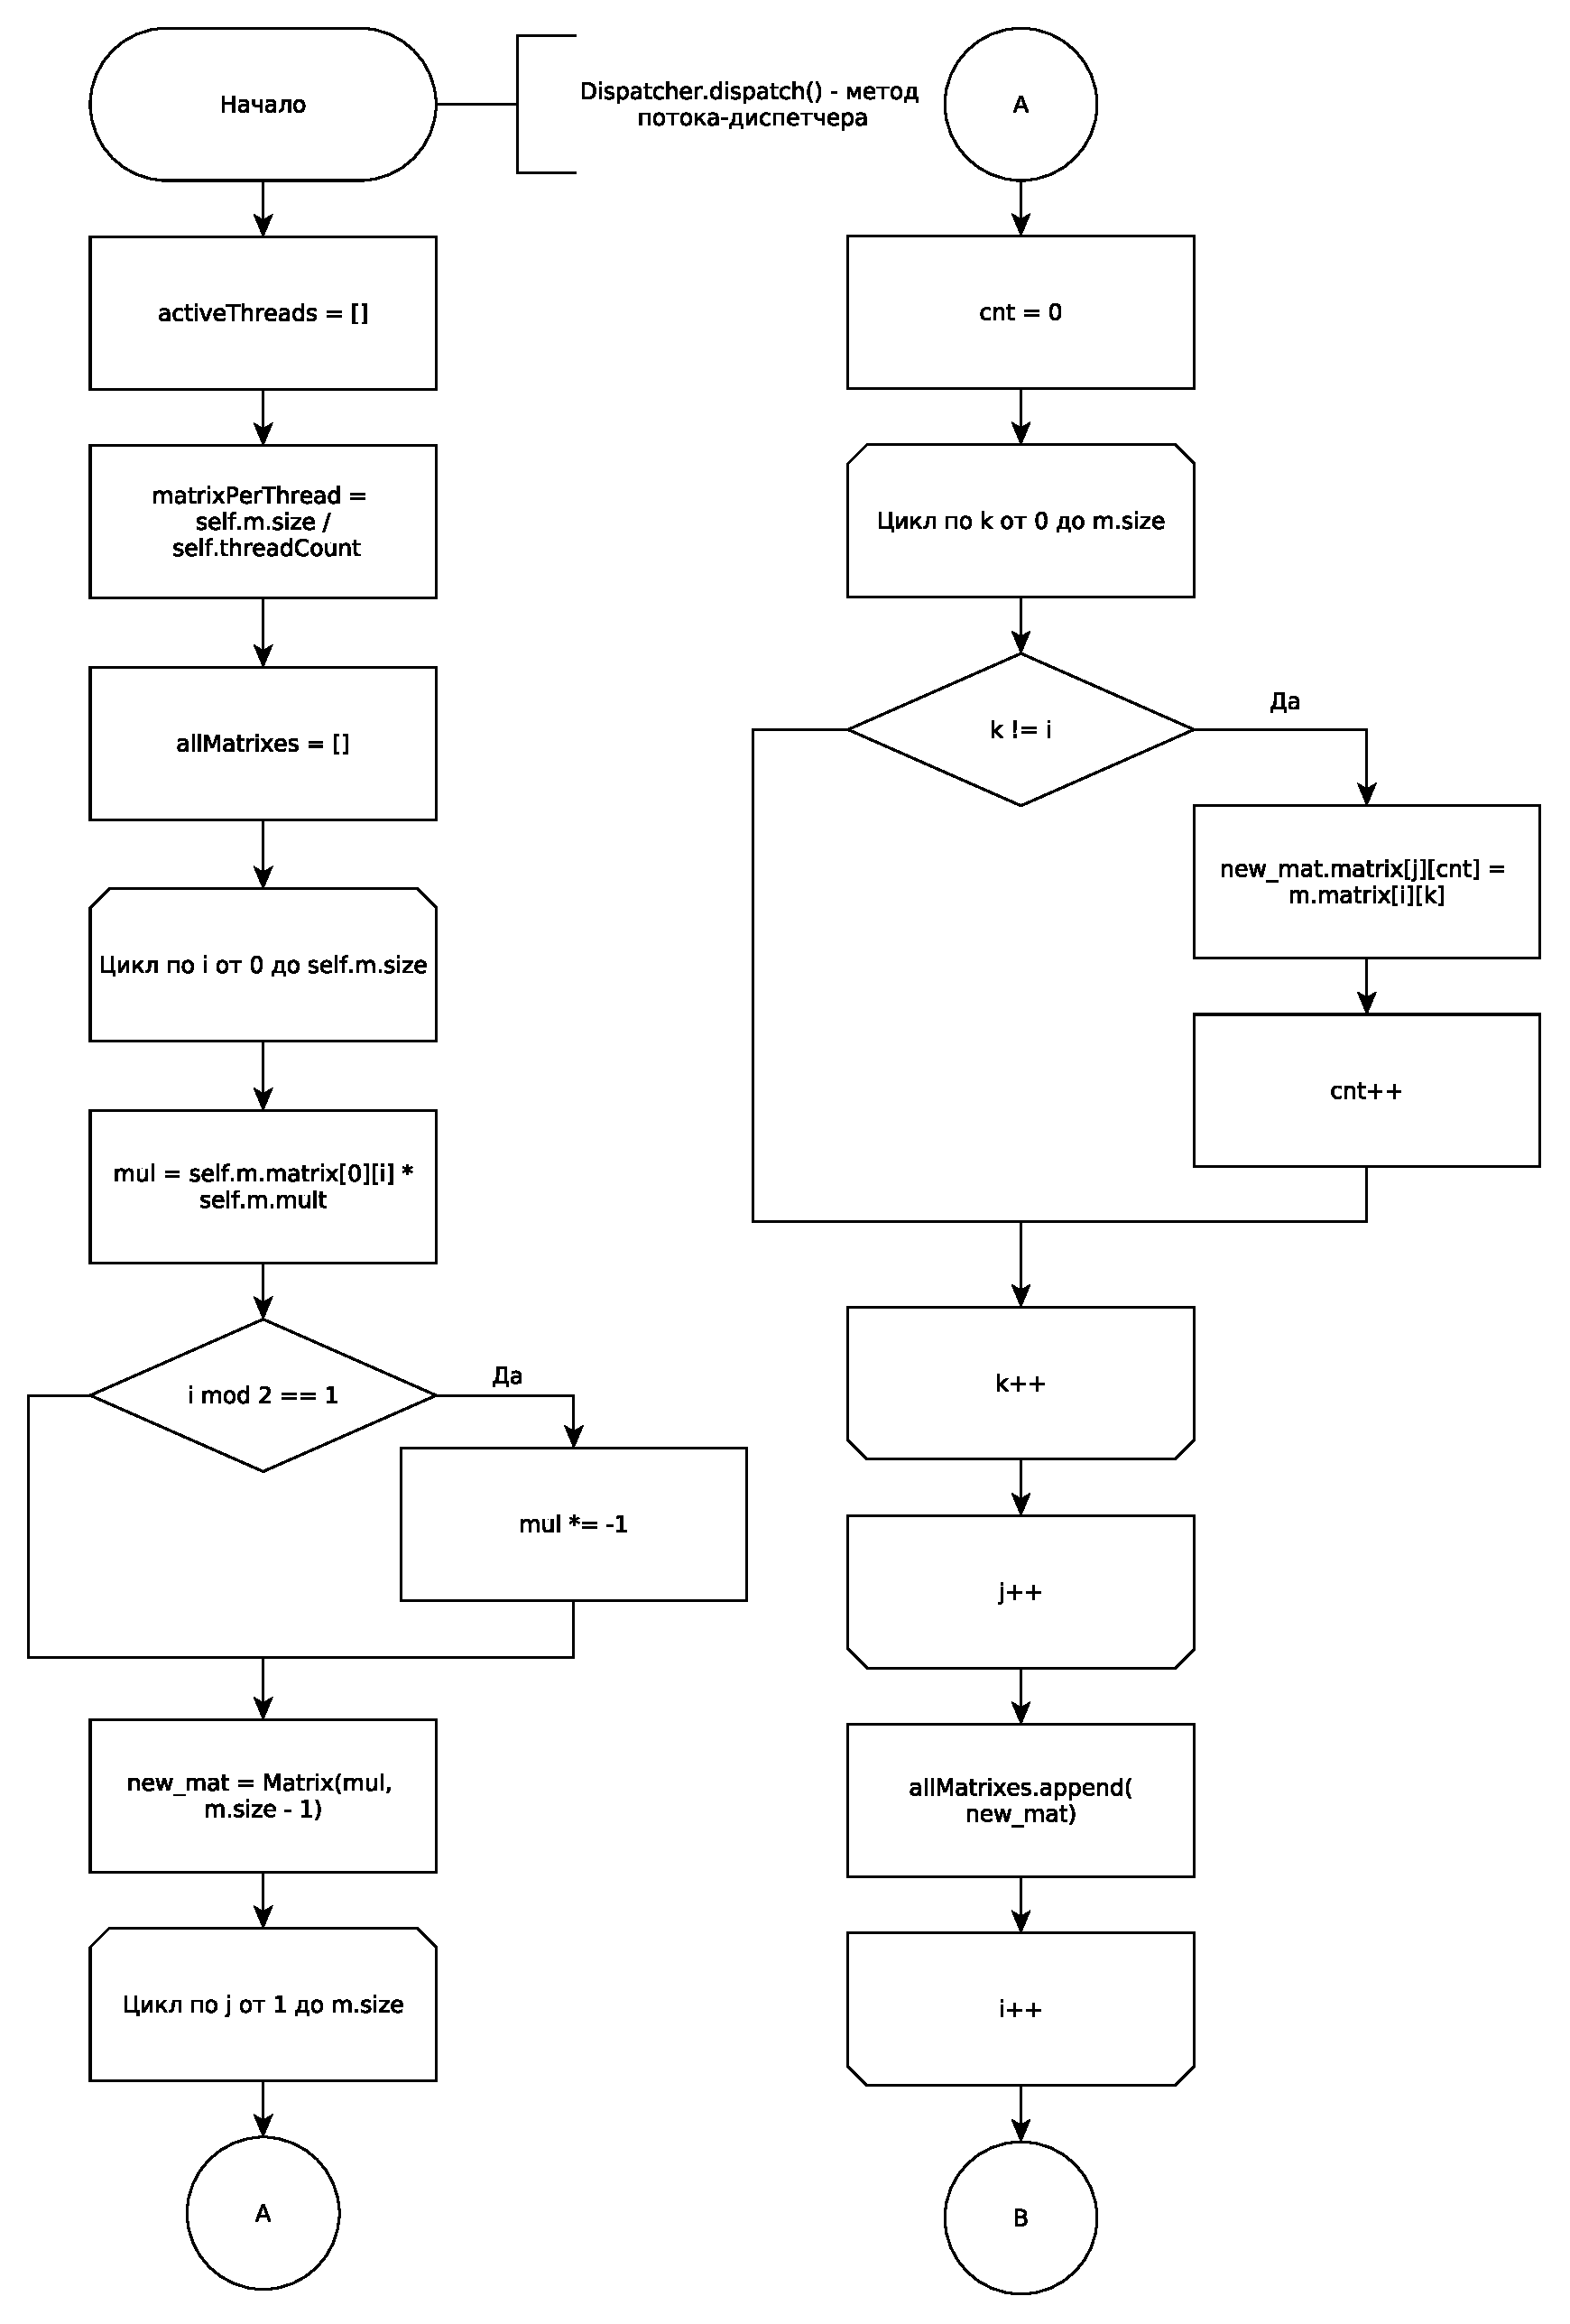
\includegraphics[width=0.85\linewidth]{img/solver_part_1}
    %	\caption{Схема алгоритма работы конвейерной обработки}
    %	\label{img:solver_1}
    %\end{figure}
    %
    \section{Структуры данных}
    Для удобства работы были выделены следующие классы:
    \begin{itemize}
    	\item UserStats
    	\begin{itemize}
    		\item поля
    		\begin{itemize}
    			\item times - массив из объектов класса Times, содержащий время поступления и выхода для каждой ленты конвейера;
    			\item user - объект класса User, содержащий данные пользователя;
    			\item current - хэш-значение пароля;
    			\item number - идентификатор объекта класса;
    		\end{itemize}
    		\item методы
    		\begin{itemize}
    			\item set\_time - установка времени входа/выхода для конкретной ленты;
    			\item get\_time - получение времени входа/выхода для конкретной ленты;
    		\end{itemize}
    	\end{itemize}
    	\item User
    	\begin{itemize}
    		\item поля
    		\begin{itemize}
    			\item login - логин пользователя;
    			\item password - пароль пользователя;
    		\end{itemize}
    		\item методы
    		\begin{itemize}
    			\item generate\_pass - генерирует случайный пароль;
    		\end{itemize}
    	\end{itemize}
    	\item Time
    	\begin{itemize}
    		\item поля
    		\begin{itemize}
    			\item time\_in - время поступления на ленту ковейера;
    			\item time\_out - время выхода с ленты конвейера;
    		\end{itemize}
    		\item методы
    		\begin{itemize}
    			\item set - установка времени поступления/выхода;
    			\item get - получение времени поступления/выхода;
    		\end{itemize}
    	\end{itemize}
    \end{itemize}
    
    Таким образом, программа генерирует заданное в программе количество пользователей и их данных, затем формирует 4 очереди и 3 ленты конвейера и запускает конвейерную обработку. После окончания выводится время конвейерной и последовательной обработки одних и тех же данных, после выводится лог, содержащий время поступления в очередь и выхода задач для каждой ленты конвейера.
    
    %\section{Классы эквивалентности}
    %Для осуществления функционального тестирования ПО были выделены следующие классы эквивалентности:
    %\begin{itemize}
    %	\item матрица, состоящая из одного элемента;
    %	\item нулевая матрица;
    %	\item единичная матрица;
    %	\item произвольная матрица, определитель которой равен нулю;
    %	\item произвольная матрица, определитель которой не равен нулю.
    %\end{itemize}
    
    \section{Вывод}
    В данном разделе приведена схема работы конвейера, выделены структуры данных для дальнейшей реализации программного обеспечения. 
    
    \chapter{Технологическая часть}
    Данный раздел содержит обоснование выбора языка и среды разработки, реализацию алгоритмов.
    
    \section{Средства реализации}
    Для реализации программы был выбран язык программирования Python~\cite{python}. Такой выбор обусловлен следующими причинами:
    \begin{itemize}
    	\item имеется большой опыт разработки;
    	\item имеет большое количество расширений и библиотек, в том числе библиотеку для работы с потоками, измерения времени, построения графиков;
    	\item обладает информативной документацией;
    \end{itemize}
    
    \section{Реализация алгоритмов}
    В листингах \ref{lst:user} - \ref{lst:master5} представлены реализации рассматриваемых алгоритмов.
    \newpage
    \captionsetup{singlelinecheck=false, justification=raggedright}
    \begin{lstlisting}[caption=Класс User, label={lst:user}]
    	PC = 'qwertyuiopasdfghjklzxcvbnm1234567890'
    	PCS = len(PC)
    	
    	class User:
    	def __init__(self, login: str = None, password: str = None):
    	if login is None:
    	self.__login = str(uuid.uuid4())
    	else:
    	self.__login = login
    	if password is None:
    	self.__password = self.__generate_pass()
    	else:
    	self.__password = password
    	
    	@staticmethod
    	def __generate_pass():
    	size = random.randint(16, 2**9)
    	a = ''
    	for i in range(size):
    	a += PC[random.randint(0, PCS - 1)]
    	return a
    	
    	@property
    	def login(self):
    	return self.__login
    	
    	@property
    	def password(self):
    	return self.__password
    \end{lstlisting}
    \newpage
    \begin{lstlisting}[caption=Класс Time, label={lst:timeClass}]
    	class Time:
    	def __init__(self):
    	self.__time_in = None
    	self.__time_out = None
    	
    	def set(self, t, is_in: bool):
    	if is_in:
    	if self.__time_in is not None:
    	raise Exception("Время поступления на ленту уже записано!")
    	self.__time_in = t
    	elif not is_in:
    	if self.__time_out is not None:
    	raise Exception("Время выхода с ленты уже записано!")
    	self.__time_out = t
    	else:
    	raise Exception("При установке параметр is_in - обязательный!")
    	
    	def get(self, is_in: bool = None):
    	if is_in is None:
    	if self.__time_out is None and self.__time_in is None:
    	raise Exception("Время не установлено!")
    	elif self.__time_out is None:
    	raise Exception("Время поступления на ленту не установлено!")
    	elif self.__time_out is None:
    	raise Exception("Время выхода с ленты не установлено!")
    	return [self.__time_in, self.__time_out]
    	elif is_in:
    	if self.__time_out is None:
    	raise Exception("Время поступления на ленту не установлено!")
    	return self.__time_in
    	else:
    	if self.__time_out is None:
    	raise Exception("Время выхода с ленты не установлено!")
    	return self.__time_out
    \end{lstlisting}
    \newpage
    \begin{lstlisting}[caption=Класс UserStats, label={lst:userStatsClass}]
    	class UserStats:
    	cnt = 0
    	
    	def __init__(self, login: str = None, password: str = None, 	do_not_init: bool = True):
    	self.__times = [Time() for _ in range(3)]
    	self.__number = self.cnt
    	if do_not_init:
    	self.user = None
    	else:
    	self.user = User(login, password)
    	self.current = ''
    	UserStats.cnt += 1
    	
    	def set_time(self, time_, stage: int, is_in: bool):
    	# is_in - True, если на вход, False, если на выход
    	# stage - номер ленты
    	if stage < 0 or stage > 2 or stage is None:
    	raise Exception("Неправильный номер ленты!")
    	self.__times[stage].set(time_, is_in)
    	
    	def get_time(self, is_in: bool = None, stage: int = None):
    	# is_in - True, если на вход, False, если на выход, обязательный
    	# stage - номер ленты, None = выдать все
    	
    	if stage is not None and (stage < 0 or stage > 2):
    	raise Exception("Неправильный номер ленты!")
    	if stage is None:
    	if is_in is None:
    	return [self.__times[i].get() for i in range(3)]
    	else:
    	return [self.__times[i].get(is_in) for i in range(3)]
    	else:
    	return self.__times[stage].get(is_in)
    	
    	def get_number(self):
    	return self.__number
    \end{lstlisting}
    \newpage
    \begin{lstlisting}[caption=Файл master.py (часть 1), label={lst:master1}]
    	def init_db(con: sqlite3.Connection):
    	cur = con.cursor()
    	cur.execute('create table if not exists users_out (login text, password text)')
    	cur.execute('create table if not exists users_in (i int, login text, password text)')
    	con.commit()
    	
    	def fill_input_db(con: sqlite3.Connection, count=30):
    	cur = con.cursor()
    	for index in range(count):
    	m = User()
    	cur.execute(f'insert into users_in (i, login, password) values ({index}, "{m.login()}", "{m.password()}")')
    	con.commit()
    	
    	def get_list_size_from_db(con: sqlite3.Connection) -> int:
    	cur = con.cursor()
    	cur.execute('select count(*) from users_in')
    	return cur.fetchone()[0]
    	
    	def clear_db(con: sqlite3.Connection):
    	cur = con.cursor()
    	cur.execute('drop table if exists users_out')
    	cur.execute('drop table if exists users_in')
    	con.commit()
    	
    	def generate_users(users_count: int) -> [UserStats]:
    	users = []
    	
    	for i in range(users_count):
    	users.append(UserStats(do_not_init=False))
    	
    	return users
    \end{lstlisting}
    \newpage
    \begin{lstlisting}[caption=Файл master.py (часть 2), label={lst:master2}]
    	def load_user(u: UserStats):
    	con = sqlite3.connect('app.db')
    	c = con.cursor()
    	c.execute(f'select login, password from users_in where i = {u.get_number()}')
    	login, password = c.fetchone()
    	u.user = User(login, password)
    	
    	def get_hashed(u: UserStats):
    	u.current = u.user.login() + 'my secret key'
    	
    	for iter in range(2000):
    	u.current = sha512((u.current + str(iter)).encode('Utf-8')).hexdigest()
    	
    	def insert(u: UserStats):
    	con = sqlite3.connect('app.db')
    	c = con.cursor()
    	c.execute(f"insert into users_out (login, password) values ('{u.user.login()}', '{u.current}')")
    	con.commit()
    	con.close()
    	
    	def tex_table(stats, stages):
    	print("\\hline")
    	print('Stage N & Task M & Start Time & End Time\\\\')
    	print("\\hline")
    	
    	for stat_num, stat in enumerate(stats):
    	for stage in range(stages):
    	times = stat.get_time(stage=stage)
    	print(
    	f'Stage: {stage + 1} & Task: {stat_num + 1} & {times[0] - start_time:.6f} & {times[1] - start_time:.6f} \\\\')
    	
    	print("\\hline")
    \end{lstlisting}
    \newpage
    \begin{lstlisting}[caption=Файл master.py (часть 3), label={lst:master3}]
    	def job(task: Callable, in_queue: SimpleQueue, out_queue: SimpleQueue, stage: int):
    	while True:
    	data: UserStats = in_queue.get()
    	
    	if data is None:
    	out_queue.put(data)
    	break
    	
    	data.set_time(time.time(), stage, True)
    	task(data)
    	data.set_time(time.time(), stage, False)
    	out_queue.put(data)
    	
    	def test_serial(users):
    	for user in users:
    	load_user(user)
    	get_hashed(user)
    	insert(user)
    	
    	if __name__ == '__main__':
    	stages_count = 3
    	
    	connection = sqlite3.connect('app.db')
    	clear_db(connection)
    	init_db(connection)
    	fill_input_db(connection)
    	
    	_users = generate_users(get_list_size_from_db(connection))
    	
    	pipeline_time = 0
    	serial_time = 0
    	cnt = 10
    	for i in range(cnt):
    	clear_db(connection)
    	init_db(connection)
    	fill_input_db(connection)
    	
    	passwords_queue = SimpleQueue()
    	salt_queue = SimpleQueue()
    \end{lstlisting}
    \begin{lstlisting}[caption=Файл master.py (часть 4), label={lst:master4}]
    	hash_queue = SimpleQueue()
    	result_queue = SimpleQueue()
    	
    	add_salter = Process(target=job, args=(load_user, passwords_queue, salt_queue, 0))
    	hasher = Process(target=job, args=(get_hashed, salt_queue, hash_queue, 1))
    	inserter = Process(target=job, args=(insert, hash_queue, result_queue, 2))
    	pipeline = [add_salter, hasher, inserter]
    	
    	for u in _users:
    	passwords_queue.put(u)
    	
    	passwords_queue.put(None)
    	start_time = time.time()
    	for worker in pipeline:
    	worker.start()
    	
    	for worker in pipeline:
    	worker.join()
    	end_time = time.time()
    	pipeline_time += end_time - start_time
    	
    	start_time_ = time.time()
    	test_serial(_users)
    	end_time_ = time.time()
    	serial_time += end_time_ - start_time_
    	
    	pipeline_time /= cnt
    	
    	print(f'Pipeline time = {pipeline_time * 1e6} mks')
    	
    	serial_time /= cnt
    	print(f'Serial time = {serial_time * 1e6} mks')
    	print('Press to get log')
    	input()
    	
    	stats = []
    \end{lstlisting}
    \newpage
    \begin{lstlisting}[caption=Файл master.py (часть 5), label={lst:master5}]
    	while not result_queue.empty():
    	stats.append(result_queue.get())
    	stats.pop()
    	
    	deltas = [[], [], []]
    	for stat in stats:
    	for stage in range(stages_count):
    	stage_stat = stat.get_time(stage=stage)
    	deltas[stage].append(stage_stat[1] - stage_stat[0])
    	
    	for stage in range(stages_count):
    	print(f'Max time on stage {stage + 1} = {max(deltas[stage]) * 1e6} mks')
    	print(f'Min time on stage {stage + 1} = {min(deltas[stage]) * 1e6} mks')
    	print(f'Avg time on stage {stage + 1} = {sum(deltas[stage]) / len(deltas[stage]) * 1e6} mks\n')
    	
    	connection.close()
    	
    	tex_table(stats, stages_count)
    \end{lstlisting}
    %
    
    \section{Выводы}
    В данном разделе была реализована конвейерная обработка данных: изменение, хеширование и сохранение паролей пользователей.
    \newpage
    
    \chapter{Экспериментальная часть}
    В данном разделе сравниваются реализованные алгоритмы, дается сравнительная оценка затрат на время.
    
    \section{Пример работы программы}
    Пример работы программы представлен на рисунке \ref{fig:ex}.
    
    \section{Технические характеристики}
    Технические характеристики устройства, на котором выполнялось исследование:
    \begin{itemize}
    	\item операционная система: Ubuntu 20.01 Linux x86\_64~\cite{ubuntu};
    	\item оперативная память: 8 Гб;
    	\item процессор: AMD Ryzen5 4500U~\cite{processor}:
    	\begin{itemize}
    		\item количество физических ядер: 6;
    		\item количество логических ядер: 6.
    	\end{itemize}
    \end{itemize}
    
    \captionsetup{singlelinecheck=true}
    \begin{figure}[H]
    	\centering
    	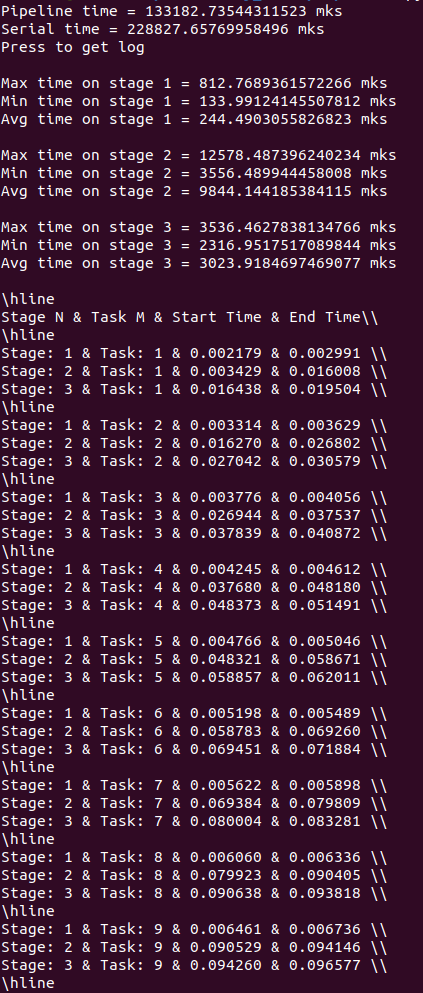
\includegraphics[width=0.55\linewidth]{img/example}
    	\caption{Пример работы программы}
    	\label{fig:ex}
    \end{figure}
    
    
    
    \section{Время выполнения алгоритмов}
    Время выполнения алгоритмов измерялось на автоматически генерируемых в необходимом количестве пользовательских данных с использованием функции time библиотеки time. Усредненные результаты 10 замеров реального времени работы приведены в таблице ниже.
    
    На рисунке \ref{fig:graph} представлена зависимость времени выполнения алгоритма в зависимости от "плана на день" - количества пользователей для обработки - на основе таблицы \ref{tab:time}. Последовательное выполнение занимает в среднем в 1.5-1.7 раз больше времени, чем конвейерное с незначительным увеличением выигрыша обработки на конвейере при увеличении количества пользователей. Таким образом, выигрыш от использования конвейерной обработки при количестве пользователей от 15 до 85 приблизительно одинаков и составляет около 1.6 раз.
    \begin{table}[H]
    	\begin{center}
    		\captionsetup{justification=raggedleft, singlelinecheck=false}
    		\caption{\label{tab:time} Время выполнения алгоритма для разного количества пользователей в микросекундах}
    		\begin{tabular}{|c| c | c|} 
    			\hline
    			Размер&Последовательное выполнение&Конвейерная обработка\\ [0.5ex]
    			\hline
    			5 &   38291.287 &  36348.152\\ 
    			\hline
    			15 &   109756.374 &   73250.5798 \\ 
    			\hline
    			25 &   181147.265 &   113172.388 \\ 
    			\hline
    			35 &   252654.957 &   152421.474 \\ 
    			\hline
    			45 &  322310.686 &  197659.373 \\ 
    			\hline
    			55 & 399007.916 & 239235.663 \\ 
    			\hline
    			65 & 461043.334 & 286625.170 \\ 
    			\hline
    			75 & 541337.20 & 321961.14 \\ 
    			\hline
    		\end{tabular}
    	\end{center}
    \end{table}
    
    \begin{figure}[H]
    	\centering
    	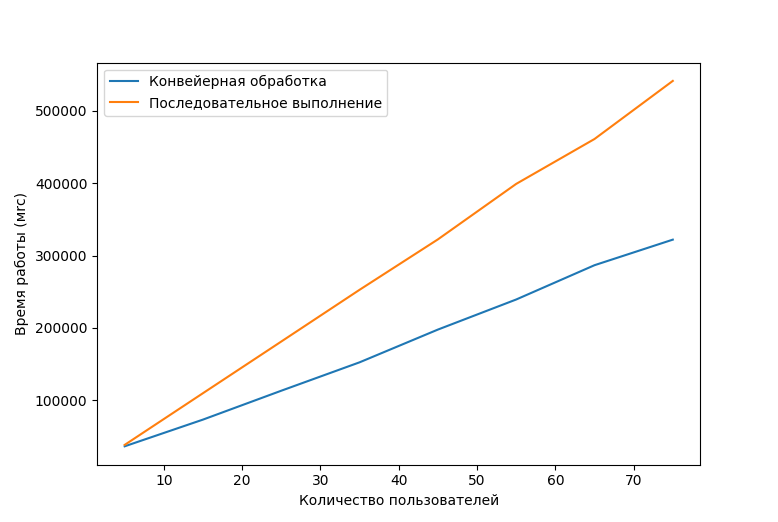
\includegraphics[width=0.9\linewidth]{img/con_vs_serial}
    	\caption{Зависимость времени выполнения от количества пользователей}
    	\label{fig:graph}
    \end{figure}
    
    \section{Тестирование}
    Для тестирования корректности работы ПО используется анализ логов. Полученная для последних 6 заявок таблица приведена ниже. На рисунке \ref{fig:maxmintime} представлены данные о максимальном, минимальном и среднем времени обработки заявок на каждой ленте конвейера.
    %
    \begin{table}[H]
    	\begin{center}
    		\captionsetup{justification=raggedleft, singlelinecheck=false}
    		\caption[]{\label{tab:tests} Полученный лог}
    		%
    		\begin{tabular}{|c|c|c|c|}
    			\hline
    			Stage N & Task M & Start Time & End Time\\
    			\hline
    			Stage: 1 & Task: 24 & 0.012759 & 0.012983 \\
    			Stage: 2 & Task: 24 & 0.096859 & 0.100533 \\
    			Stage: 3 & Task: 24 & 0.100766 & 0.103546 \\
    			\hline
    			Stage: 1 & Task: 25 & 0.013081 & 0.013289 \\
    			Stage: 2 & Task: 25 & 0.100624 & 0.104318 \\
    			Stage: 3 & Task: 25 & 0.104567 & 0.107468 \\
    			\hline
    			Stage: 1 & Task: 26 & 0.013381 & 0.013590 \\
    			Stage: 2 & Task: 26 & 0.104418 & 0.108121 \\
    			Stage: 3 & Task: 26 & 0.108363 & 0.111242 \\
    			\hline
    			Stage: 1 & Task: 27 & 0.013669 & 0.017236 \\
    			Stage: 2 & Task: 27 & 0.108238 & 0.111867 \\
    			Stage: 3 & Task: 27 & 0.112061 & 0.114830 \\
    			\hline
    			Stage: 1 & Task: 28 & 0.017447 & 0.017701 \\
    			Stage: 2 & Task: 28 & 0.111984 & 0.115609 \\
    			Stage: 3 & Task: 28 & 0.115740 & 0.118498 \\
    			\hline
    			Stage: 1 & Task: 29 & 0.017766 & 0.017931 \\
    			Stage: 2 & Task: 29 & 0.115671 & 0.119328 \\
    			Stage: 3 & Task: 29 & 0.119419 & 0.122284 \\
    			\hline
    			Stage: 1 & Task: 30 & 0.017987 & 0.018134 \\
    			Stage: 2 & Task: 30 & 0.119397 & 0.123048 \\
    			Stage: 3 & Task: 30 & 0.123159 & 0.126240 \\
    			\hline
    		\end{tabular}
    	\end{center}
    \end{table}
    \captionsetup{singlelinecheck=true}
    \begin{figure}[H]
    	\centering
    	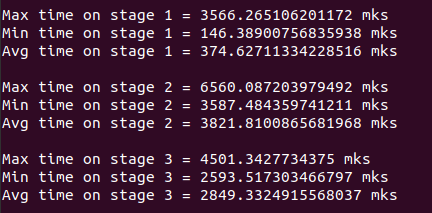
\includegraphics[width=0.65\linewidth]{img/maxmintime}
    	\caption{Время выполнения заявок на каждой из лент конвейера}
    	\label{fig:maxmintime}
    \end{figure}
    
    
    \section{Выводы}
    В данном разделе были проведены измерения времени, затрачиваемого на загрузку данных о пользователе из базы данных, хеширование пароля и сохранения в базу данных полученного хэша.
    Для размера входной очереди конвейера, принадлежащего интервалу [5, 85], выигрыш по сравнению с последовательной обработкой составил приблизительно 1.5-1.7 раз с небольшими колебаниями при увеличении количества пользователей.
    \newpage
    
    \addcontentsline{toc}{chapter}{Заключение}
    \chapter*{Заключение}
    В процессе выполнения лабораторной работы было реализовано асинхронное взаимодействие потоков на примере конвейерной обработки данных. В качестве конвейера рассмотрена работа с логинами и паролями пользователей: загрузка из базы данных, многократное хеширование хеш-функцией SHA-512 с добавлением "солей" и сохранение полученных данных в базу данных.
    
    Было исследовано время выполнения выше обозначенного алгоритма. В результате было выявлено, что в среднем для количества пользователей от 5 до 85 выигрыш от использования конвейерной обработки составляет 1.6 раз с небольшим увеличением при увеличении количества пользователей.
    
    \newpage
    \addcontentsline{toc}{chapter}{Список литературы}
    \addcontentsline{toc}{chapter}{Литература}

    \bibliographystyle{utf8gost705u}  % стилевой файл для оформления по ГОСТу
    \bibliography{report_5}          % имя библиографической базы (bib-файла)

\end{document}